\newif\ifPAPER  
%\PAPERtrue % select either slide or note
\PAPERfalse  

\newcommand{\mytitle}{\title{Ideal $\tau$ tagging with TMVA multivariate data-analysis toolkit}}

\newcommand{\myauthor}{
\author{A.~Heikkinen} 
\affiliation{Helsinki Institute of Physics, P.O. Box 64, FIN-00014 University of Helsinki (Finland)}
}
\mytitle
\newcommand{\codeAlgorithm}[1]{
\addcontentsline{toc}{section}{Résumé}
\begin{center}\fbox{\parbox{12cm}{\bf #1}}\end{center}}

\newcommand{\cppintro}[1]{
\lstset{language=C,
caption= #1 ,
label=listing:boundary}}

\def\cppstart{\begin{lstlisting}}
\def\cppend{\end{lstlisting}}

\newif\ifCITENOTE 
\CITENOTEtrue

\ifPAPER

\else   % Slides ---------------------------------------------------------------

\documentclass[slidestop,compress,xdvips,10pt]{beamer} 
\usetheme{Antibes}
\usecolortheme{lily}
\usepackage{graphicx}
\usepackage{hyperref}
\usepackage{listings}
\usepackage{verbatim} % for comment
\transglitter[direction=315]
\xdefinecolor{ahcol}{rgb}{0.2, 0.4, 0.1}
\xdefinecolor{olive}{cmyk}{0.64,0,0.95,0.4}
\colorlet{structure}{green!60!black} % for color substitution
\usepackage{color} % for definecolor
\definecolor{light-gray}{gray}{0.95}
\definecolor{dark-gray}{gray}{0.30}
\definecolor{orange}{rgb}{1,0.5,0}
\definecolor{dark-blue}{cmyk}{1,0.5,0.5,0}

\hypersetup{
    a4paper, % page format
    pdftitle={My Title},                  % Title
    pdfsubject={Subject of the document}, % Subject 
    pdfauthor={Author name},              % Author
    pdfkeywords={list of keywords},       % Keywords
    plainpages=true, %
    colorlinks,       % links are colored
    urlcolor=dark-blue,    % color of external links
    linkcolor=dark-blue,    % color of internal links
    citecolor=black,  % color of links to bibliography
    bookmarksnumbered
}

\usecolortheme[named=ahcol]{structure}
\useoutertheme{myinfolines}
\useinnertheme{rounded}
\setbeamercolor{alerted_text}{fg=blue}
\makeatother
\beamertemplatetransparentcoveredhigh
\mytitle
\author{\underline{A.~Heikkinen}\footnote{aatos.heikkinen@cern.ch}, P.~Kaitaniemi, V. Karim\"{a}ki,
 R.~Kinnunen,  M.~J.~Kortelainen, T.~Lamp\'{e}n, S.~Lehti, T.~Lind\'{e}n, and L.~Wendland 
%\footnote{Helsinki Institute of Physics, P.O. Box 64, FIN-00014 University of Helsinki, Finland.}
}
\institute{Helsinki Institute of Physics, P.O. Box 64, FIN-00014 University of Helsinki, Finland.}
%\author{Aatos Heikkinen 
%\footnote{Helsinki Institute of Physics, Helsinki, Finland.
%{\tt aatos.heikkinen@cern.ch}} and Ivica Puljak 
%\footnote{University of Split - FESB, Split, Croatia}
%}
\graphicspath{{.}{figures/}}
\begin{document}
\frame{\titlepage}
\begin{comment}
\end{comment}

\section{Outline}

\begin{comment}
We report our experience on using ROOT package TMVA for
multivariate data analysis, for a problem of $\tau$ tagging in the
framework of heavy charged MSSM Higgs boson searches at the LHC.



With a generator level analysis, 
we investigate how in the ideal case $\tau$ tagging could be performed and 
hadronic $\tau$ decays separated from the
hadronic jets of QCD multi-jet background present in LHC experiments. 

A successful separation of the Higgs signal from the background 
requires a rejection factor of $10^5$ or better against the QCD background. 

The $\tau$ tagging efficiency and background rejection are studied with various MVA classifiers.
\end{comment}

\subsection{}
\frame{
\frametitle{Outline}

\begin{itemize}
\item {\bf Motivation}: our experience on using ROOT package TMVA for multivariate data analysis
\footnote{T.~Lampen {\em et. al.}, Testing TMVA software in b-tagging 
                  for the search of MSSM Higgs bosons at the LHC,
CHEP’07, Journal of Physics: Conference Series 119 (2008) 032028}


\item {\bf Use case:} $\tau$ tagging in the
framework of heavy charged MSSM Higgs boson searches at the LHC

\item {\bf Goal:} 
to investigate how in the ideal case (no detector effects) $\tau$ tagging could be performed and 
signal $\tau$s separated from the background

\vspace{0.5cm}

\item {\bf Data:} a generator level Pythia/Tauola data for  14 TeV  p-p collisions
\begin{itemize}
\item Signal: hadronic $\tau$ decay
\item Background: hadronic QCD multi-jets
\end{itemize}

\vspace{0.2cm}
\item {\bf Method/Results:} The $\tau$ tagging efficiency and 
background rejection are studied with various MVA classifiers
\begin{itemize}
\item Moderate customisation was required to map our problem into the TMVA framework
\end{itemize}
\end{itemize}
\vspace{0.5cm}


%Introduction to concept of \href{http://en.wikipedia.org/wiki/Probability}{probability}

\vspace{0.5cm}

}

\section{Data}
\frame{
\frametitle{Data}
{\bf The data for  QCD background} was generated using Pythia8.108 for LHC 14 TeV p-p collisions.

\vspace{0.1cm}
{\bf The signal}  was generated with Pythia6.4.19,
and required to consist only of genuine $\tau$ jets from the 
(heavy charged) MSSM $H^{\pm} \rightarrow \tau^{\pm}\nu_{\tau}$ decay 
with $\tau$ polarization simulated with Tauola 2.6\footnote{D.P. Roy, Phys. Lett. B 459 607-614}.
\\($m_{H_{\pm}}=200 GeV/c^2$, $\tan\beta = 30$, max. $m_H$ SUSY scenario \footnote{\href{http://arxiv.org/pdf/hep-ph/9912223}{arXiv:hep-ph/9912223}}.)


%(jet ET, jet eta, charged track isolation (minimum track pT), 
%ECAL isolation (maximum ET allowed in isolation annulus), 
%neutral hadron rejection (i.e. track p matching to HCAL energy deposition), Rtau variable)

%TMVA:ssa asetetaan lisaksi vaatimus, 
%etta jetissa on vain yksi jalki 
%(seka signaali- etta taustajeteille); 
%lisaksi TMVA:ssa vaaditaan "signal tau jets are MC matched to H+ -> tau nu".

\vspace{0.1cm}
Our analysis is based on the following variables:


\begin{center}
\begin{tabular}{l*{2}{l}r}
\hline
Variable                                                 & Name                   \\
\hline
Jet $E_T$                                                & {\tt jetEt}            \\
Jet $\eta$                                               & {\tt jeteta}           \\
Track isolation ($\Delta$R=0.50)                         & {\tt isolMaxPt50}      \\
ECAL isolation ($\Delta$R=0.04-0.50)                     & {\tt ecalIsolEt10\_50} \\
Neutral hadron rejection                                 & {\tt hcalRatio}        \\
(i.e. track p matching to HCAL energy deposition)        &                        \\
$R_{\tau}$ = p(leading track) / E(jet)                   & {\tt rtau}             \\
\hline
\end{tabular}
\end{center}


%\begin{center}
%\begin{tabular}{l*{2}{l}r}
%\hline
%Variable                                    & Selection                  \\
%\hline
%Jet $E_T$                                   & {\tt jetEt>119}            \\
%Jet $\eta$                                  & {\tt |jeteta|<1.7}         \\
%Leading track $p_T$                         & {\tt ldgPt>20}             \\
%Track isolation ($\Delta$R=0.50)            & {\tt isolMaxPt50<1.0}      \\
%Signal track (1-prog)                       & {\tt signalTracks==1}      \\
%ECAL isolation ($\Delta$R=0.04-0.50)        & {\tt ecalIsolEt10\_50<1.8} \\
%Electron rejection                          & {\tt hcalRatio>-0.9}       \\
%Neutral hadron rejection                    & {\tt hcalRatio<0.1}        \\
%$\tau$-helicity correlations \footnote{D.P. Roy, Phys. Lett. B 459 607-614}  &                            \\

%$R_{\tau}$ = p(leading track) / E(jet)      & {\tt rtau>0.8}             \\
%\hline
%\end{tabular}
%\end{center}

%\cite{roy00a}:
}

\frame{
\frametitle{Production and Preselection Cuts}

At Monte Carlo level the following preselection cuts were used:
\begin{itemize}
\item {\tt jetEt $>$ 100}
\item {\tt abs(jeteta) $<$ 2.2} {\color{dark-blue}(Fig.~1)}
\item Jet leading track p$_T$ $>$ 20 GeV, matching cone 0.1
\item Isolation:

\begin{itemize} 
\item track p$_T$ $>$ 0.5
\item abs(track $\eta$) $<$ 2.5
\item abs(d$_{IP}$-z) $<$ 0.2
\item around the leading track:
\begin{itemize}
\item signal cone $\Delta$R $<$ 0.04 
\item isolation cone 0.04-0.5 
\end{itemize} 
\item signal tracks 0, 1 or 2
\item isolation tracks 0 or 1
\end{itemize} 
\end{itemize} 

Further, before analysis we choose:
\begin{itemize}
\item 1-prong signal final states ({\tt signalTracks==1} )
\item MC matched $\tau$ jets coming from $H^{\pm}$ ({\tt tauDecayType==4})
\end{itemize}


%    listan MC-tasolla tehdyista leikkauksista tuottokoodissa? Ts. jet ET, eta, jne.
%Signaali: H+,pythia prosessit 401,402, mA=200GeV, tanb = 30, mhmax SUSY scenario, 
%Pythia 6.4.19 + Tauola, 
%H+ pakotettu hajoamaan tau+nu lopputilaan, 
%ainastaan hadroniset 1-prong taut valittu.
%Tausta: QCD 120 < pthat < 170 GeV, Pythia 8.108
%CM Energy 14 TeV
%

%Viela efficiencyt:
%
%H+:
%   allEvents                    100000
%   excludeDecays                98816
%   preSelection                 23902
%
%   allEvents                    200000
%   excludeDecays                197586
%   preSelection                 47866
%QCD:
%   allEvents                    9.97999e+07
%   excludeDecays                9.97999e+07
%  preSelection                 1.63405e+06

}

%\subsection{Data}
\frame{
\frametitle{}
\vspace{1cm}
\begin{figure}[h]
 \begin{minipage}{5.5cm}
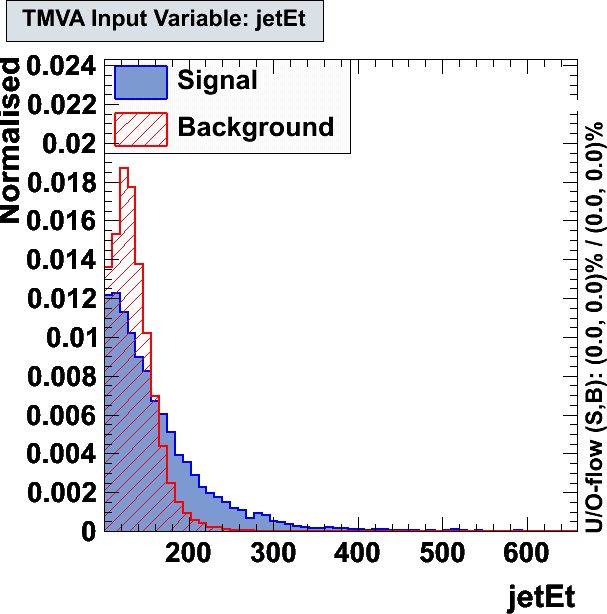
\includegraphics[width=1.0\textwidth]{images/jetet.png}
\end{minipage}
 \hfill
\begin{minipage}{5.5cm}
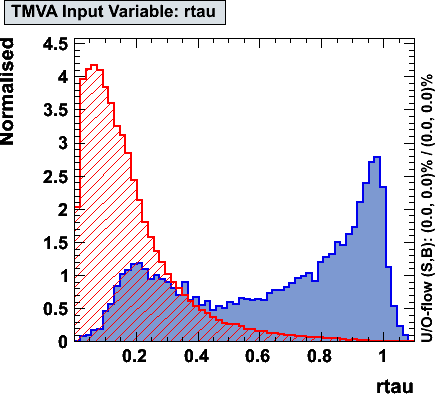
\includegraphics[width=1.0\textwidth]{images/rtau.png}
\end{minipage}
%\begin{minipage}{3.0cm}

{\color{dark-blue} Fig.~1: Example of data used in $\tau$ tagging: \\
distribution of jet $E_T$ ({\tt jetEt}) and $R_{\tau}$ ({\tt rtau})}.
%\end{minipage}
\label{fig:variables}
\end{figure}
}

\section{TMVA}
\frame{
\frametitle{TMVA - Toolkit for Parallel Multivariate Data Analysis}

ROOT-integrated TMVA is a framework the training, testing and performance evaluation
of multivariate classification techniques.

\vspace{0.5cm}
TMVA works in {\bf transparent factory mode 
to guarantee an unbiased performance comparison between the classifiers}, such as:

\begin{itemize}
\item Rectangular cut optimisation
\item Projective likelihood estimation (PDE approach)
%\item Multidimensional probability density estimation (PDE - range-search approach)
\item Multidimensional k-nearest neighbour classifier
\item Linear discriminant analysis (H-Matrix and Fisher discriminants)
%\item Function discriminant analysis (FDA)
%\item Predictive learning via rule ensembles (RuleFit)
\end{itemize}
 

\vspace{0.5cm}
In this presentation, we are focusing to following classifiers applied to problem of $\tau$ tagging:
\begin{itemize}
\item Artificial neural networks (ANN)
\item Boosted/Bagged decision trees (BDT)
\item Support Vector Machine (SVM) 
\end{itemize}
}

\section{Customisation of TMVA}
\begin{frame}[fragile]
%\frame{
\frametitle{Customisation of TMVA for $\tau$ tagging 1/2}
\vspace{0.5cm}
We added:
\begin{itemize}
\item Evaluation of event efficiencies with {\tt TMVA::Reader}, taking into account
   the MC-level preselection efficiencies and TMVA preselection efficiencies

\item Timing profiling with {\tt TStopwatch}

\vspace{0.5cm}
\item Signal (event) efficiency at background (event) efficiency levels $10^{-5}$ and $10^{-6}$
\item Signal (jet) efficiency at $10^{-5}$,  background (jet) efficiency

\end{itemize}
%\scriptsize
%\begin{verbatim}
%\end{verbatim}
%\normalsize
\end{frame}


\begin{frame}[fragile]
%\frame{
\frametitle{Customisation of TMVA for $\tau$ tagging 2/2}
\scriptsize
\begin{verbatim}
MyEvaluate : Testing classifiers in order to obtain signal/background efficiencies for EVENTS
MyEvaluate : (not jets, which are the input to TMVA)
MyEvaluate :
MyEvaluate : -----------------------------------------------------------------------------
MyEvaluate :              |             Events             |               Jets
MyEvaluate :              |   Signal   eff       Bkg   eff |   Signal  eff       Bkg  eff
MyEvaluate : -----------------------------------------------------------------------------
MyEvaluate : Generated    :   200000        89799840       |      N/A            N/A
MyEvaluate : Event presel :    47866 0.239   1470627 0.016 |   206079        4345182
MyEvaluate : TMVA  presel :    35615 0.744   1087375 0.739 |    35615 0.17   2230315 0.51
MyEvaluate : Total presel :          0.178           0.012 |
MyEvaluate : -----------------------------------------------------------------------------
MyEvaluate :
MyEvaluate : Thus 1e-5 overall bkg event efficiency corresponds to 8.3e-04 bkg event
MyEvaluate : efficiency by TMVA.
MyEvaluate :
MyEvaluate : Signal and background event efficiencies have been scaled with the preselection
MyEvaluate : event efficiencies
MyEvaluate : Evaluation results ranked by best signal efficiency at 1e-5
MyEvaluate : -----------------------------------------------------------------------------
MyEvaluate : MVA              Signal event efficiency at bkg event efficiency (error):
MyEvaluate : Methods:         @B=1e-6      @B=1e-5      @B=1e-4      @B=1e-3      @B=0.01
MyEvaluate : -----------------------------------------------------------------------------
MyEvaluate : SVM_Gauss_2_5  : 0.0212(007)  0.0556(012)  0.1096(016)  0.1670(019)  0.1774(020)
MyEvaluate : -----------------------------------------------------------------------------
\end{verbatim}
\normalsize
\end{frame}

\section{Results}
\frame{
\frametitle{Results - Neural Networks 1/2}

\begin{itemize}
\item {\bf ANN:} Of the three Multilayer Perceptrons (MLP) implementations supported by TMVA
we used {\tt kMLP} ({\tt TMVA::Types::kMLP}).
%\item {\bf Varaibles:} {\tt jetEt, jeteta, log(isolMaxPt50), log(ecalIsolEt10\_50), log(hcalRatio), rtau}
\item {\bf Variables:} {\tt jetEt, jeteta, isolMaxPt50, ecalIsolEt10\_50, hcalRatio, rtau}


\vspace{0.5cm}
\item {\bf Training:} Data for 6-13-1 MLP configuration with neurons of tanh type we trained 1k cycles
\begin{itemize}
\item 5k signal jets and 40k background jets 
\end{itemize}

\vspace{0.5cm}
\item {\bf Testing:} Rest of the data was used for testing \\(35k signal and 2230k background events)
\begin{itemize}
\item Systematic uncertainty was estimated by repeating the full analysis with independent background data
\end{itemize}
\end{itemize}

% / {\tt kCFMlpANN} (Clermont-Ferrand) / {\tt kTMlpANN}) 
%we focused on recommended neural network implementation .

%\vspace{0.5cm}

}

\frame{
\frametitle{Results - Neural Networks 2/2}
\vspace{1cm}
\begin{figure}[h]
 \begin{minipage}{5.5cm}
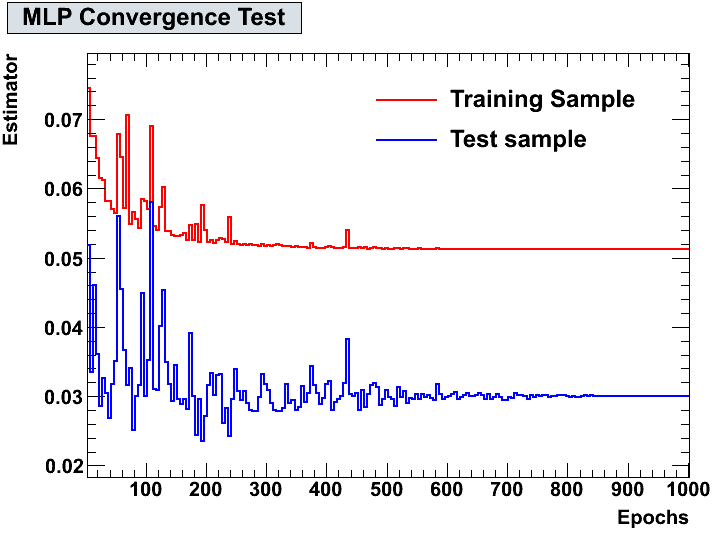
\includegraphics[width=1.0\textwidth]{images/MLPConvergenceTest.png}
\end{minipage}
 \hfill
\begin{minipage}{5.5cm}

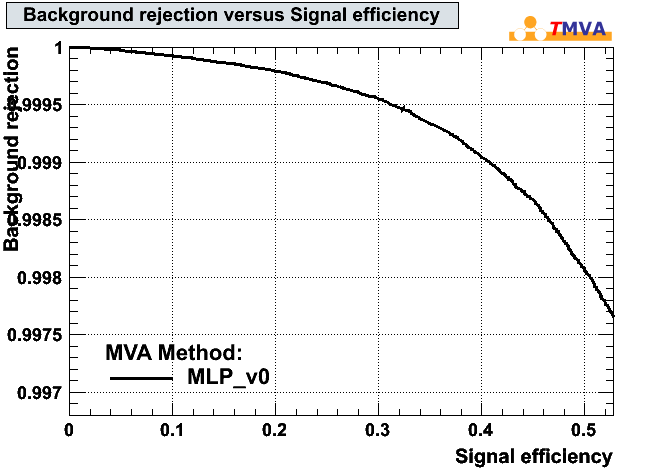
\includegraphics[width=1.0\textwidth]{images/roc.png}
\end{minipage}
%\begin{minipage}{3.0cm}

{\color{dark-blue} Fig.~2: Convergence of ANN over 1000 training cycles and background rejection vs. signal efficiency.}
%\end{minipage}
\label{fig:variables}
\end{figure}
\begin{center}
\begin{tabular}{l*{2}{l}r}
\hline
Signal efficiency (\%)  & Background eff. \\
\hline
4.6$\pm$0.1 (stat.) $\pm$ 0.1 (syst.)       & $10^{-5}$               \\
1.3$\pm$0.3 $\pm$ 0.1       & $10^{-6}$               \\
\hline
\end{tabular}
\end{center}

}


\frame{
\frametitle{Results - Boosted Decision Trees}

A decision tree is a binary tree classifier. 
Repeated left/right (yes/no) decisions are performed on a single variable at a time.:
\begin{itemize}
\item The phase space is split into regions that are classified as signal or
background, depending on the majority of training events that end up in the final leaf nodes
\end{itemize}

\vspace{0.3cm}
{\bf Boosted Decision Trees (BDT) implemented in TMVA 
represents an extension to a single decision tree to several decision trees}
derived from the same training sample by reweighting events.

\vspace{0.3cm}
New combined classifier has stabilized response with respect to fluctuations in the training sample.

% LW 090318
%BDT:lla olen tehnyt joitakin ajoja ja huomannut, 
%etta tulokset ovat hyvin samankaltaisia ajosta riippumatta 
%ja myoskin opetusjoukosta riippumatta. 
%Taydella opetusjoukolla ja evaluointijoukolla 
%saan signaalieffisienssiksi 7.8 % (epavarmuus lienee korkeintaan +-0.1%), 
%kun taustan rejektio on 1e5. 1e6 -rejektiolla signaalin effisienssi on 3.9 % 
%(epavarmuus n. +- 0.1%). Aikaa yhteen ajoon menee n. 4 h 50 min.
%

%With full teaching data and testing sample signal efficiency
%BDT was found to behave stable and only small fluctiations:
%%was found to be 7.8$\pm$0.1\% for background rejection $10^5$.
%%(For BG rejection $10^6$ signal efficiency was 3.9$\pm$0.1\%.)

\vspace{0.3cm}
For our $\tau$ tagging problem the BDT method was found to give {\bf stable results 
with only small fluctuations}:
\begin{center}
\begin{tabular}{l*{2}{l}r}
\hline
Signal efficiency (\%)  & Background eff. \\
\hline
7.8$\pm$0.1        & $10^{-5}$               \\
3.9$\pm$0.1        & $10^{-6}$               \\
\hline
\end{tabular}
\end{center}
}



%The definition of the efficiency {\bf optimization problem} has an important role in the case of SVM:
%\begin{itemize}
%\item The signal jet efficiency has a maximum in a different point of parameter space than event efficiency
%\item Same is true for  different levels of background efficiency
%\end{itemize}

%\begin{center}
%\begin{tabular}{l*{3}{l}r}
%\hline
%Signal efficiency (\%)  & & Background eff. \\
%Background (BG) sample 1 & BG sample 2 & \\
%\hline
%5.56$\pm$0.12  & 5.50$\pm$0.12        & $10^{-5}$               \\
%2.1$\pm$0.07   & 2.18$\pm$0.07        & $10^{-6}$               \\
%\hline
%\end{tabular}
%\end{center}

%\footnote{Independent background sample}


%\item SVM achieves $5.56\;\%$ signal event efficiency at $10^{-5}$
%  background event efficiency level, $2.11\;\%$ for $10^{-6}$ bkg eff
%  with same parameters%C=5, sigma=2
%\item Training with bkg sample 2 gives $5.50\;\%$ signal eff for
%  $10^{-5}$ bkg eff, from which we could estimate the systematic
%  uncertainty from the selection of the training data to be at least
%  on ther order of $0.06\;\%$; for $10^{-6}$ the signal eff is
%  $2.18\;\%$, and the systematic uncertainty would become $0.07\;\%$
%  \begin{itemize}
%  \item Statistical uncertainty in $10^{-5}$ case is $0.12\;\%$, and
%    $10^{-6}$ case $0.07\;\%$
%  \end{itemize}

%\end{itemize}



\frame{
\frametitle{Results - Support Vector Machine 1/2}

%Example distribution of the SVM classifier output is in Fig.~\ref{fig:mkSvmGauss}
\begin{figure}[h]
 \begin{minipage}{4.5cm}
SVM were {\bf trained with 5k signal jets} and {\bf 40k background jets}:
\vspace{0.5cm}
  \begin{itemize}
  \item The training in SVM scales as {\em O(\# of events in training data$^2$)}  
\item In practice training took $\sim$1 h 
  \end{itemize}

\end{minipage}
\hfill
 \begin{minipage}{6.5cm}
  \begin{center}
    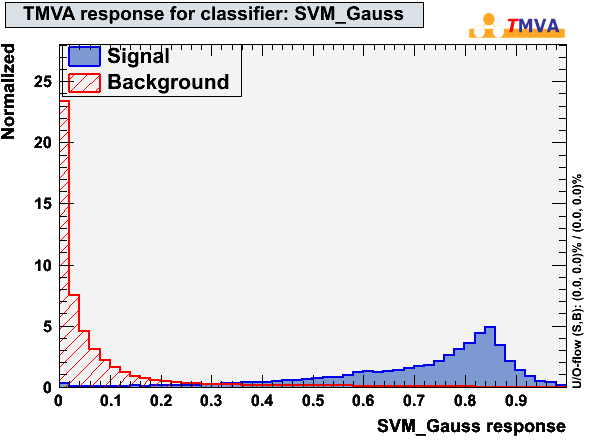
\includegraphics[width=1.0\textwidth]{images/mk_svm_gauss}
  \end{center}

{\color{dark-blue}The output of the SVM classifier with a Gaussian kernel}.

\end{minipage}
\label{fig:mkSvmGauss}
\end{figure}
}

\frame{
\frametitle{Results - Support Vector Machine 2/2}
\begin{figure}[h]
  \begin{center}
    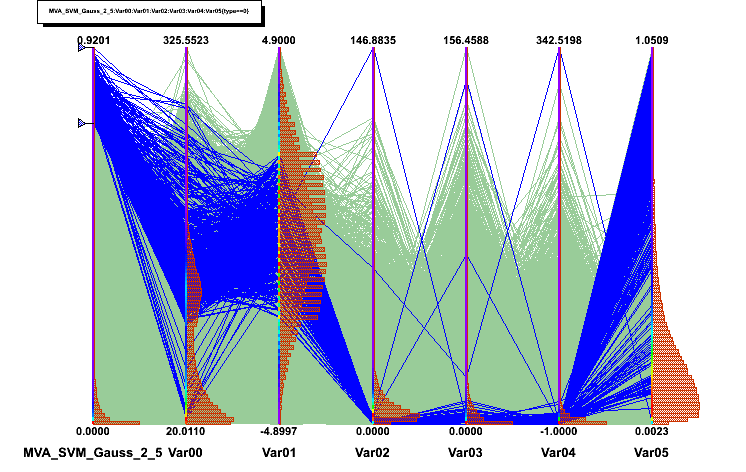
\includegraphics[width=0.7\textwidth]{images/svm_parallels}
  \end{center}
{\color{dark-blue}Parallel coordinates -plot indicating poorly classified events.}
  \label{fig:parallel}
\end{figure}
%Independent data samples were used to estimate systematic uncertainty:
\begin{center}
\begin{tabular}{l*{2}{l}r}
\hline
Signal efficiency (\%)  & Background eff. \\
\hline
5.56$\pm$0.12 $\pm$ 0.06        & $10^{-5}$               \\
2.11$\pm$0.07 $\pm$ 0.07        & $10^{-6}$               \\
\hline
\end{tabular}
\end{center}
}

\section{Conclusions}
\frame{
\frametitle{Conclusions}
\begin{itemize}
\item Since CHEP'07, TMVA has matured and is now fully integrated to ROOT
\begin{itemize}
\item An {\bf interface for adding new classifiers} is provided
\end{itemize}
\item Some customisation was needed to cast our problem into the TMVA framework
\vspace{0.5cm}
\item Multivariate data-analysis techniques show a promise in $\tau$ tagging:
\begin{itemize}
\item At  $10^{-5}$ background efficiency, TMVA classifiers have 4.6-7.8~\% signal efficiency
\end{itemize}
\item Finally, we have defined areas where our approach can be improved (e.g. using extra variables), 
and are planning to perform additional research on this

\end{itemize}
}
\bibliographystyle{alpha}  % Options plain, unsrt, alpha, abbrv
\bibliography{chep09} %10 p

\end{document}

\fi %slides



